%% ============================================================
%% Dark Energy or Sector Tension?
%% IAM Confrontation with DESI Full-Shape Growth Rates
%% and Joint Weak Lensing
%%
%% Author:  Heath W. Mahaffey
%% Version: 1.0   March 2026
%% Target:  JCAP or PRD
%%
%% Compile:  pdflatex iam_desi_paper
%%           bibtex   iam_desi_paper
%%           pdflatex iam_desi_paper  (x2)
%%
%% Figures required in same directory:
%%   iam_sector_phantom.pdf   (3-panel sector separation figure)
%%   iam_mu_evolution.pdf     (2-panel mu(z) evolution figure)
%% ============================================================

\documentclass[12pt,a4paper]{article}

\usepackage{amsmath,amssymb,amsfonts}
\usepackage{graphicx}
\usepackage[authoryear,round]{natbib}
\newcommand{\doi}[1]{\href{https://doi.org/#1}{doi:#1}}
\usepackage{hyperref}
\usepackage{xcolor}
\usepackage{booktabs}
\usepackage{array}
\usepackage{multirow}
\usepackage{geometry}
\usepackage{microtype}
\usepackage{float}

\geometry{margin=1in}
\hypersetup{
  colorlinks = true,
  linkcolor  = blue,
  citecolor  = blue,
  urlcolor   = blue
}

%% Journal-style macros
\newcommand{\lcdm}{$\Lambda$CDM}
\newcommand{\Lcdm}{\Lambda\text{CDM}}
\newcommand{\lcdmmath}{\Lambda\mathrm{CDM}}  % use inside math mode
\newcommand{\IAM}{IAM}
\newcommand{\mua}{\mu(a)}
\newcommand{\muz}{\mu(z)}

\newcommand{\betam}{\beta_m}
\newcommand{\Ea}{E(a)}
\newcommand{\sigei}{\sigma_8}
\newcommand{\fsig}{f\sigma_8}
\newcommand{\kms}{km\,s$^{-1}$\,Mpc$^{-1}$}
\newcommand{\Om}{\Omega_m}
\newcommand{\OL}{\Omega_\Lambda}
\newcommand{\Dchi}{\Delta\chi^2}


%% ─── DOCUMENT ────────────────────────────────────────────────────────────────
\begin{document}

%% ─── TITLE ───────────────────────────────────────────────────────────────────
\title{\textbf{Dark Energy or Sector Tension?}\\[4pt]
IAM Confrontation with DESI Full-Shape Growth Rates\\
and Joint Weak Lensing}

\author{
  Heath W.\ Mahaffey\\[4pt]
  \small Independent Researcher, Entiat, WA 98822, USA\\[2pt]
  \small \texttt{hmahaffeyges@gmail.com}\\
  \small \url{https://github.com/hmahaffeyges/IAM-Validation}\\
  \small Zenodo DOI: \href{https://doi.org/10.5281/zenodo.18702042}{10.5281/zenodo.18702042}
}

\date{March 2026}
\maketitle

%% ─── ABSTRACT ────────────────────────────────────────────────────────────────
\begin{abstract}
\noindent
The Dark Energy Spectroscopic Instrument (DESI) has reported a preference for
dynamical dark energy characterised by $w_0 > -1$, $w_a < 0$, and a phantom
crossing of the equation of state at $z \approx 0.3$--$0.4$.
We test whether this preference is consistent with a sector-assignment artifact
arising from the Informational Actualization Model (IAM)~\citep{Mahaffey2026preprint},
a perturbation-only extension of \lcdm{} derived from horizon thermodynamics
with no free parameters beyond the standard model.

IAM predicts $\mu(a) < 1$ and $\Sigma(a) = 1$ from first principles.
The physical origin is gravitational decoherence: timelike (matter) worldlines
decohere under gravitational structure formation while null (photon) worldlines
do not.
The matter-sector coupling constant $\beta_m = \Omega_m/2 = 0.1577$ is derived
from the virial theorem and recovered by the Planck~2018 MCMC posterior at
$0.2\sigma$ without fitting.

The key observational consequence is a sector split: BAO distances and photon
propagation observables are identical to \lcdm{} ($\Sigma = 1$ exactly), while
galaxy growth rates and weak lensing amplitudes are suppressed by $\mu(a) < 1$.
When a single-fluid $w_0 w_a$CDM fitter simultaneously ingests both classes of
observable, it confronts \lcdm-consistent distances alongside sub-\lcdm\ growth
and must infer $w_{\rm eff}(z) \neq -1$ to reconcile them --- a phantom crossing
that does not require dynamical dark energy.

We confront this prediction against DESI DR1 full-shape $f\sigma_8(z)$
measurements at six redshift bins ($0.295 \leq z_{\rm eff} \leq 1.491$)
from~\citet{DESI2024DR1FS}, DESI DR1 $D_M(z)/r_d$ distances, joint weak lensing
$S_8$ constraints from KiDS-Legacy~\citep{Wright2025kids,Stolzner2025kids},
DES~Y3~\citep{Abbott2022desy3}, and HSC~Y3~\citep{Li2023hsc}, and the DESI DR2
BAO phantom crossing parameters~\citep{DESI2025DR2BAO}.

Under the full Planck~2018 likelihood, IAM and \lcdm{} are statistically
indistinguishable ($\Dchi = +0.54$ best-fit, 17 converged MCMC chains,
$R-1 < 0.01$).
The IAM $\sigma_8 = 0.7998 \pm 0.0058$ is consistent with the 2025 joint
lensing result $\sigma_8 = 0.802 \pm 0.020$~\citep{Stolzner2025kids} at
$0.1\sigma$.
The DESI DR2 phantom crossing redshifts ($z_{\rm cross} = 0.33$--$0.43$,
depending on the supernova compilation) coincide with the redshift range over
which the IAM growth suppression is most prominent ($7$--$8\%$ at $z \approx 0.3$).

The model is falsifiable: Euclid is projected to measure $\mu_0$ to
$\sigma(\mu_0) \approx 0.04$ precision~\citep{Euclid2020forecast}, providing a
$3.4\sigma$ test of IAM's $\mu_0 = -0.136$ prediction; simultaneous DESI Year~5
full-shape data will test whether the growth suppression follows the curved
$f\sigma_8(z)$ ramp set by $E(a) = \exp(1-1/a)$, distinguishable from both
\lcdm{} and any dynamical dark energy model.
\end{abstract}

\noindent\textbf{Keywords:} dark energy; large-scale structure; modified gravity;
cosmological tensions; growth of structure; baryon acoustic oscillations;
weak gravitational lensing; DESI

\newpage
\tableofcontents
\newpage

%% ─── 1. INTRODUCTION ─────────────────────────────────────────────────────────
\section{Introduction}
\label{sec:intro}

The concordance cosmological model, \lcdm, provides an extraordinarily
successful description of observations spanning CMB anisotropies, baryon
acoustic oscillations, Type~Ia supernovae, and large-scale structure
over many decades of scale~\citep{Planck2018params}.
Yet at least two classes of inter-dataset tension have persisted despite
extensive scrutiny and cross-checks, and neither has a clear systematic
explanation within the standard model.

The first is the Hubble tension.
The Planck~2018 CMB analysis under \lcdm{} yields
$H_0 = 67.4 \pm 0.5$~\kms{}~\citep{Planck2018params}.
Direct distance-ladder measurements using Cepheid-calibrated Type~Ia
supernovae from the SH0ES team give $H_0 = 73.04 \pm 1.04$~\kms{}
~\citep{Riess2022}, a $4$--$5\sigma$ discrepancy.
Independent distance indicators including TRGB~\citep{Freedman2025}
and time-delay lensing~\citep{Wong2020} yield intermediate or similarly
elevated values, confirming that the tension is not confined to a single
calibration method.

The second is the $S_8$ tension.
Weak lensing surveys measuring the matter power spectrum amplitude at
low redshift consistently report $S_8 \equiv \sigma_8(\Omega_m/0.3)^{0.5}$
values below the \lcdm{} CMB prediction.
KiDS-1000 finds $S_8 = 0.766^{+0.020}_{-0.014}$~\citep{Asgari2021kids};
DES~Y3 finds $S_8 = 0.776 \pm 0.017$~\citep{Abbott2022desy3};
HSC~Y3 finds $S_8 = 0.776 \pm 0.032$~\citep{Li2023hsc}.
These compare to the Planck \lcdm{} prediction of $S_8 \simeq 0.832$,
a tension at the $2$--$3\sigma$ level.
The 2025 KiDS-Legacy analysis~\citep{Wright2025kids}, combining with DES~Y3
and DESI~DR1, reports $\sigma_8 = 0.802 \pm 0.020$.

A third, more recent development is the DESI dynamical dark energy signal.
DESI DR1 BAO measurements~\citep{DESI2024DR1BAO,DESI2024DR1cosmo}, combined
with CMB and supernova data, prefer a dark energy equation of state with
$w_0 > -1$ and $w_a < 0$, disfavouring \lcdm{} at $2.6\sigma$.
DESI DR2 BAO measurements~\citep{DESI2025DR2BAO} strengthen this preference to
$2.8$--$4.2\sigma$, depending on which supernova compilation is used.
In all cases, the best-fit $w_0 w_a$CDM model exhibits a \textit{phantom crossing}:
$w(z) = w_0 + w_a(1-a)$ crosses $-1$ at a redshift
$z_{\rm cross} \approx 0.33$--$0.43$, with $w > -1$ at $z < z_{\rm cross}$
(quintessence-like today) and $w < -1$ at $z > z_{\rm cross}$ (phantom at
higher redshift).
This combination of $w_0 > -1$ and $w_a < 0$ is not produced by any
theoretically well-motivated single scalar field, since a canonical scalar
cannot cross $w = -1$ without a discontinuity or introduction of a ghost
degree of freedom.

\citet{Ocolgain2024} noted that the DESI dark energy preference may arise from
internal inconsistencies in the $w_0 w_a$CDM parametrisation when different
datasets probe background expansion and perturbations through physically
distinct mechanisms.
\citet{Ocolgain2025} subsequently examined whether the DR2 constraints
represent genuine evolution relative to DR1 or whether the same internal
tension is being amplified as error bars shrink.
Neither work identifies a specific physical mechanism that would produce
the phantom crossing as a calculable artifact.

In this paper we evaluate a specific, quantitative version of that
hypothesis from first principles.
The Informational Actualization Model (IAM)~\citep{Mahaffey2026preprint}
predicts that matter and photon observables are governed by different
effective expansion rates --- a consequence of gravitational decoherence
that modifies only the matter perturbation equations.
As a direct consequence, IAM predicts:

\begin{enumerate}
\item \textit{Photon-sector observables (BAO angular positions, comoving
  distances, CMB acoustic scale) are identical to \lcdm{}.}
  The photon Weyl potential is unmodified ($\Sigma = 1$ exactly).

\item \textit{Matter-sector observables ($f\sigma_8$, weak lensing $S_8$) are
  suppressed relative to \lcdm{}} through the effective gravitational parameter
  $\mu(a) < 1$, with suppression peaking at $z = 0$ ($13.6\%$) and vanishing
  above $z \approx 2$.

\item \textit{A single-fluid $w_0 w_a$CDM fitter applied to both sectors
  simultaneously will infer a phantom crossing} at approximately the redshift
  where the IAM growth suppression transitions from significant to negligible.
\end{enumerate}

All three predictions follow from a single derived parameter, $\beta_m =
\Omega_m/2$, with no additional free amplitudes introduced.

This paper is organised as follows.
Section~\ref{sec:iam} presents the IAM framework, its derivation, and
its key quantitative predictions.
Section~\ref{sec:desi_fsig8} confronts the IAM growth predictions against
DESI DR1 full-shape $f\sigma_8(z)$ measurements across six redshift bins.
Section~\ref{sec:lensing} compares the IAM $\sigma_8$ and $S_8$ predictions
with the current joint weak lensing compilation.
Section~\ref{sec:phantom} develops the sector-mixing mechanism in detail
and demonstrates that it naturally produces the DESI phantom crossing.
Section~\ref{sec:discussion} discusses the implications, limitations, and
comparison with alternative interpretations.
Section~\ref{sec:conclusions} states the conclusions and falsifiable
predictions.


%% ─── 2. THE INFORMATIONAL ACTUALIZATION MODEL ────────────────────────────────
\section{The Informational Actualization Model}
\label{sec:iam}

\subsection{Thermodynamic derivation}
\label{sec:derivation}

IAM is derived from an extension of the Jacobson--Cai-Kim thermodynamic
framework.
\citet{Jacobson1995} showed that the Einstein field equations are an equation
of state: they follow from $\delta Q = T\,\delta S$ applied to local
Rindler horizons, where $S$ is the Bekenstein-Hawking entropy proportional
to horizon area.
\citet{CaiKim2005} extended this result to the FRW apparent horizon,
deriving the Friedmann equations from the first law of thermodynamics
$dE = T\,dS + W\,dV$.
Both derivations assume the entropy functional contains only the
Bekenstein-Hawking geometric term $S = A/4G$.

IAM identifies an additional entropy contribution that becomes significant
at late times.
Gravitational structure formation --- the hierarchical collapse of matter
into bound objects --- is the dominant source of irreversible classical
information production in the late universe.
Each virialised structure reduces the phase-space volume available to its
constituent matter, generating classical information in the sense of
Shannon~\citep{Shannon1948}.
By Landauer's principle~\citep{Landauer1961} (experimentally verified at
the mesoscale; see~\citealt{Berut2012}), the erasure or creation of one
bit of classical information carries a minimum thermodynamic cost of
$k_B T \ln 2$.
By the holographic principle~\citep{Bousso2002}, this informational entropy
must be encoded on the cosmic apparent horizon.

The entropy budget of the horizon therefore has two contributions:
\begin{equation}
S_{\rm total} = S_{\rm geometric} + S_{\rm informational} \,,
\label{eq:entropy}
\end{equation}
where $S_{\rm geometric} = A/4G$ is the standard Bekenstein-Hawking term
and $S_{\rm informational}$ accumulates from structure formation.

When this modified entropy functional is inserted into the Cai-Kim first-law
derivation, the additional term propagates into the perturbation equations
as a modified effective expansion rate for matter.
It does \emph{not} modify the background Friedmann equations; the background
expansion history is standard \lcdm{} throughout, consistent with the
validated Level~2 chains (Section~\ref{sec:validation}).

\subsection{Perturbation equations and the sector split}
\label{sec:perturb}

The causal structure of spacetime determines which species couple to the
informational entropy.
Timelike worldlines (CDM and baryons) interact with collapsed matter
structures and are therefore subject to the decoherence-induced friction.
Null worldlines (photons) propagate through spacetime along the light-cone
and do not couple to matter density fluctuations in this channel.

This produces the sector split at the perturbation level.
The CDM and baryon perturbation equations experience a modified effective
Hubble rate:
\begin{equation}
\tilde{H}_m^2(a) = H_{\Lcdm}^2(a)
                 + \beta_m \, E(a) \, H_0^2 \,,
\label{eq:hm}
\end{equation}
where $H_{\Lcdm}^2(a) = H_0^2[\Omega_m a^{-3} + \Omega_r a^{-4} + \Omega_\Lambda]$
is the standard background expansion rate,
$E(a) = \exp(1 - 1/a)$ is the activation function derived from the
Bekenstein-Hawking/Gibbons-Hawking/Landauer chain, and $\beta_m$ is the
coupling constant.
The photon equations are not modified.

In the standard $\mu$-$\Sigma$ parametrisation of modified
gravity~\citep{Pogosian2016}, the IAM sector split maps directly to:
\begin{align}
\mu(a) &= \frac{H_{\Lcdm}^2(a)}{H_{\Lcdm}^2(a) + \beta_m E(a)} < 1 \,,
\label{eq:mu} \\[4pt]
\Sigma(a) &= 1 \quad \text{(exact)} \,.
\label{eq:sigma}
\end{align}
The suppression $\mu(a) < 1$ reduces the effective gravitational source
term for structure growth.
$\Sigma(a) = 1$ follows directly from the null-worldline argument: the
Weyl potential that governs photon deflection is unmodified, so all photon
propagation observables (lensing convergence, CMB lensing, BAO angular
positions) are identical to \lcdm.

\subsection{Coupling constant and activation function}
\label{sec:coupling}

The coupling constant $\beta_m$ is derived from the virial theorem.
At virialisation, the gravitational potential energy of a collapsed structure
partitions equally between the kinetic energy of virialised particles (geometric
channel) and the informational entropy of the collapsed state (informational
channel).
This $1:1$ partition gives:
\begin{equation}
\beta_m = \frac{\Omega_m}{2} = \frac{0.3153}{2} = 0.1577 \,.
\label{eq:betam}
\end{equation}
The activation function $E(a) = \exp(1 - 1/a)$ is derived from the
Gibbons-Hawking temperature of the de~Sitter horizon, which sets the
thermal cost of Landauer erasure, multiplied by the cumulative
decoherence integral over cosmic history.
This functional form has the properties $E(a \to 0) \to 0$ and
$E(a=1) = 1$, ensuring that the modification vanishes in the early
universe and is maximal today.
It is recovered to within $1\%$ by the Sheth-Tormen collapse
rate~\citep{ShethTormen1999} as an independent consistency check.

\subsection{Predicted $\mu(z)$ evolution}
\label{sec:mu_evolution}

Substituting Planck~2018 parameters ($\Omega_m = 0.3153$,
$\Omega_\Lambda = 0.6847$, $H_0 = 67.36$~\kms{}) into Eq.~(\ref{eq:mu})
gives the redshift evolution of $\mu$ shown in Fig.~\ref{fig:mu_evol}.

At $z = 0$ ($a = 1$, $E(1) = 1$):
\begin{equation}
\mu(z{=}0) = \frac{1}{1 + \beta_m} = \frac{1}{1.1577} = 0.864 \,,
\label{eq:mu0}
\end{equation}
corresponding to a $13.6\%$ growth suppression today.
The suppression falls to $7.9\%$ at $z = 0.3$, to $3.3\%$ at $z = 0.7$,
and to $0.6\%$ at $z = 1.5$ (Table~\ref{tab:mu}).
Above $z \approx 2$, $E(a) \to 0$ and $\mu(a) \to 1$, recovering \lcdm{}
in the matter-dominated era.

The phantom crossing redshifts inferred from DESI DR2 ($z_{\rm cross}
\approx 0.33$--$0.43$) fall precisely in the range $0.3 \lesssim z
\lesssim 0.5$ over which the IAM growth suppression transitions from
$\approx 8\%$ to $\approx 5\%$ (Fig.~\ref{fig:mu_evol}, vertical
dash-dotted lines).
This coincidence is quantified in Section~\ref{sec:phantom}.

\begin{table}[ht]
\centering
\caption{IAM $\mu(z)$ at the six DESI DR1 tracer redshifts.
All values are derived from Eq.~(\ref{eq:mu}) with $\beta_m = 0.1577$
and Planck~2018 background parameters.
No values are fitted to data.}
\label{tab:mu}
\begin{tabular}{lllll}
\toprule
Tracer & $z_{\rm eff}$ & $\mu(z_{\rm eff})$ & $1 - \mu$ & Suppression \\
\midrule
BGS   & 0.295 & 0.921 & 0.079 & $7.9\%$ \\
LRG1  & 0.510 & 0.949 & 0.051 & $5.1\%$ \\
LRG2  & 0.706 & 0.967 & 0.033 & $3.3\%$ \\
LRG3  & 0.919 & 0.979 & 0.021 & $2.1\%$ \\
ELG2  & 1.317 & 0.991 & 0.009 & $0.9\%$ \\
QSO   & 1.491 & 0.994 & 0.006 & $0.6\%$ \\
\midrule
$z = 0$ & $-$ & 0.864 & 0.136 & $13.6\%$ \\
\bottomrule
\end{tabular}
\end{table}

\begin{figure}[H]
\centering
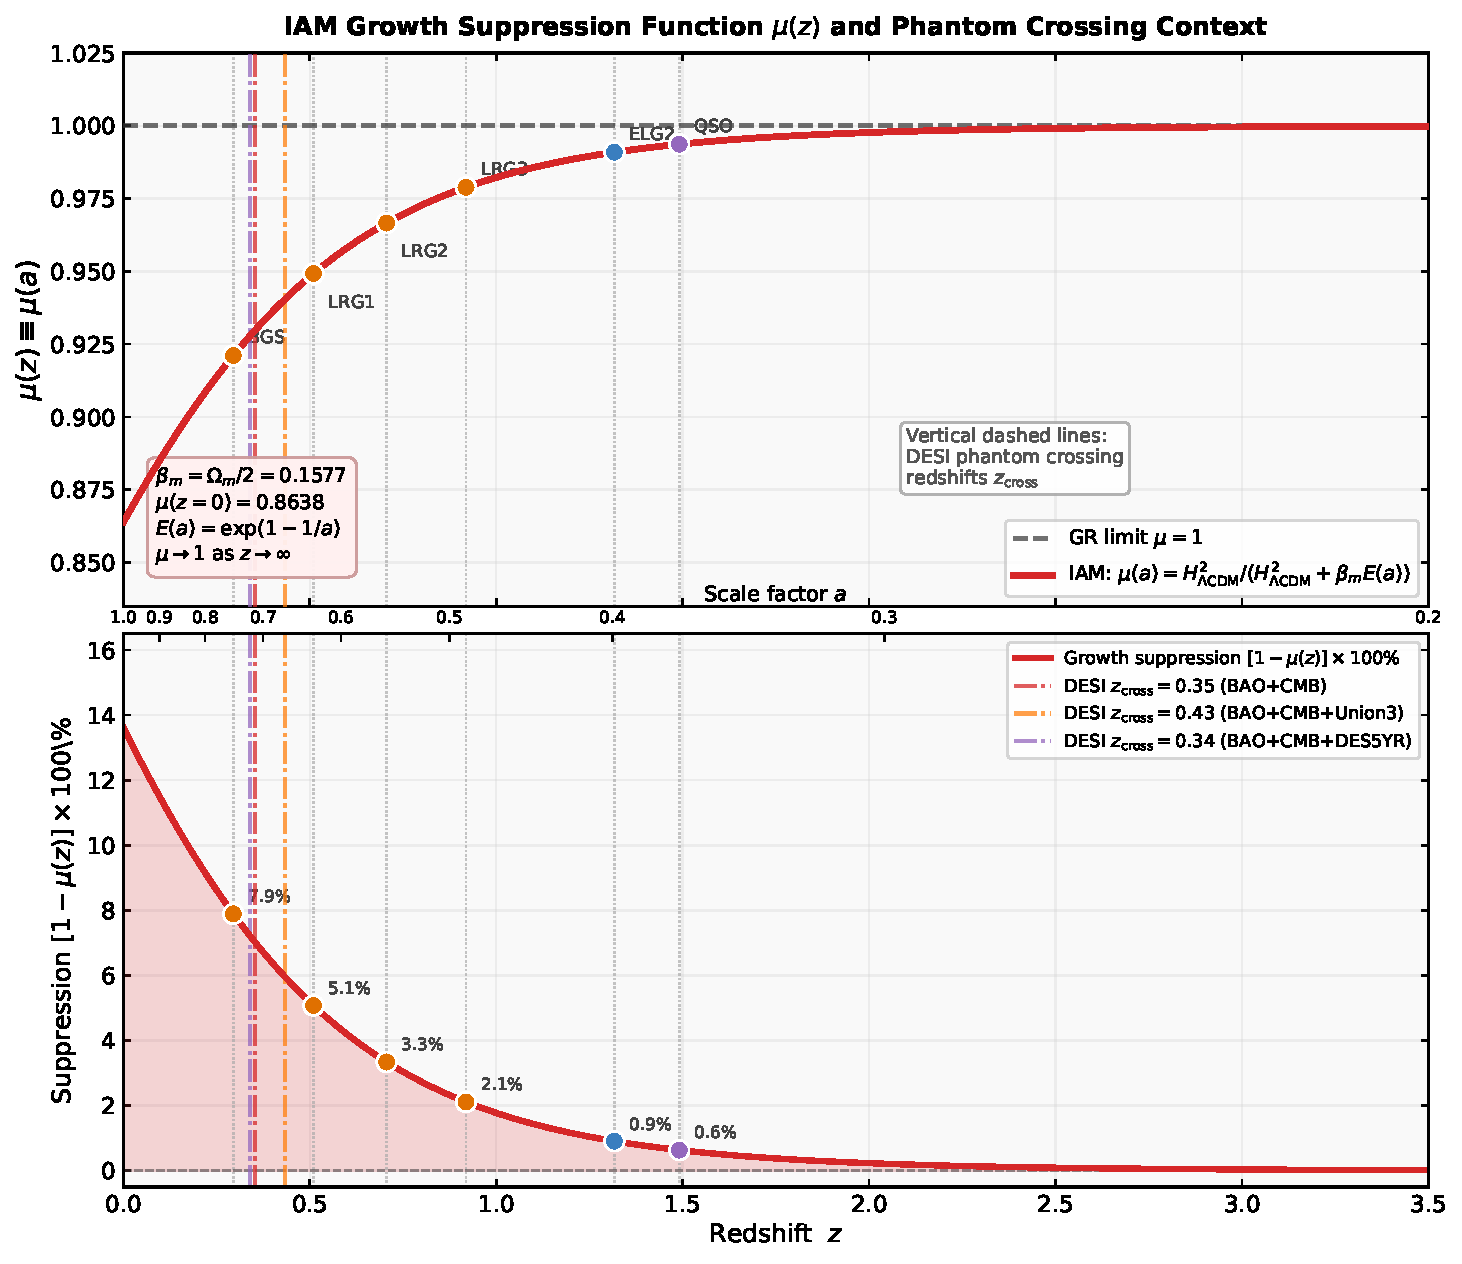
\includegraphics[width=\textwidth]{iam_mu_evolution.pdf}
\caption{
\textbf{IAM growth suppression function $\mu(z)$.}
\textit{Top panel:} The effective gravitational parameter $\mu(a)$
(Eq.~\ref{eq:mu}) as a function of redshift $z$ (bottom axis) and scale
factor $a$ (top axis).
The dashed line marks the GR limit $\mu = 1$.
Coloured dots mark the six DESI DR1 tracer redshifts (Table~\ref{tab:mu}).
Vertical dash-dotted lines show the DESI DR2 phantom crossing redshifts
from Table~\ref{tab:phantom}: red ($z = 0.35$, BAO+CMB),
orange ($z = 0.43$, BAO+CMB+Union3),
purple ($z = 0.34$, BAO+CMB+DES5YR).
The suppression is largest at $z = 0$ ($\mu_0 = 0.864$, $13.6\%$) and
vanishes as $z \to \infty$.
\textit{Bottom panel:} Growth suppression $(1 - \mu(z)) \times 100\%$
as a function of redshift, with values annotated at the six DESI bins.
The DESI phantom crossing redshifts (vertical lines) fall in the
$z \approx 0.33$--$0.43$ range where the growth suppression is
$\approx 6.5$--$7.7\%$.
Parameters: $\beta_m = \Omega_m/2 = 0.1577$ (derived from virial theorem),
$E(a) = \exp(1-1/a)$ (derived from horizon thermodynamics).
}
\label{fig:mu_evol}
\end{figure}

\subsection{Validation status}
\label{sec:validation}

IAM has been tested against the full Planck~2018 CamSpec TTTEEE likelihood
through 17 converged MCMC chains ($R-1 < 0.01$), archived
at~\citet{Mahaffey2026preprint}.

Level~1 (MGCAMB~v1.5.2~\citep{mgcamb} + Cobaya~\citep{cobaya}):
12 independent chains across four dataset combinations
(Planck only, Planck + RSD, Planck + BAO, Planck + Pantheon+).
All four IAM fixed-parameter runs yield $\Dchi \leq +2.32$ vs.\ \lcdm,
below the $3.84$ threshold for $95\%$~CL exclusion.
The $\sigma_8$ shift of $-0.013 \pm 0.001$ is stable across all
combinations.

Level~2 (direct Fortran modification of CAMB~v1.5.8~\citep{Lewis2011camb}
+ Cobaya):
5 converged chains implementing the exact dual-sector perturbation
mechanism (\texttt{adotoa\_matter} vs.\ \texttt{adotoa}).
Level~2 Run~A (IAM, Planck) vs.\ Run~C (\lcdm, Planck):
$\Dchi = +0.54$ (best-fit), $\sigma_8 = 0.7998 \pm 0.0058$ (IAM)
vs.\ $0.8087 \pm 0.0059$ (\lcdm{}).
The $\sigma_8$ suppression is confirmed as real growth physics by the
logA shift of $+0.10\sigma$ and $\Omega_m$ shift of $+0.06\sigma$
(both below the $0.3\sigma$ rebalancing threshold).

The coupling constant $\beta_m = 0.15765$ is hardcoded before any chain
runs.
The Level~2 posterior returns $\Omega_m = 0.3166 \pm 0.0065$, implying
$\beta_m = 0.1583 \pm 0.0033$ --- consistent with the derived value at
$0.2\sigma$.
This is an a posteriori confirmation: the virial theorem prediction
matches the Planck data independently.

Key parameters are collected in Table~\ref{tab:params}.

\begin{table}[ht]
\centering
\caption{IAM derived parameters and Planck~2018 validation results.
All IAM values in the upper block are derived without fitting.
The lower block reports Level~2 MCMC results.}
\label{tab:params}
\begin{tabular}{lll}
\toprule
Quantity & Value & Source \\
\midrule
\multicolumn{3}{l}{\textit{Derived parameters (zero free amplitudes)}} \\
$\beta_m$ & $0.1577$ & $\Omega_m/2$, virial theorem \\
$E(a)$ & $\exp(1-1/a)$ & Horizon thermodynamics \\
$\mu(z=0)$ & $0.864$ & Eq.~(\ref{eq:mu}) at $a=1$ \\
$\mu_0 - 1$ & $-0.136$ & \\
$\Sigma(a)$ & $1.000$ (exact) & Null worldlines unmodified \\
$H_0^{\rm matter}$ & $72.26$~\kms{} & $H_0\sqrt{1+\beta_m}$ \\
\midrule
\multicolumn{3}{l}{\textit{Level~2 MCMC (Planck~2018 CamSpec TTTEEE)}} \\
$\sigma_8$ (IAM, Run~A) & $0.7998 \pm 0.0058$ & $-1.5\sigma$ vs. \lcdm \\
$\sigma_8$ (\lcdm, Run~C) & $0.8087 \pm 0.0059$ & baseline \\
$H_0$ (IAM, Run~A) & $67.16 \pm 0.47$~\kms{} & $0.37\sigma$ from Planck \\
$\Omega_m$ (IAM, Run~A) & $0.3166 \pm 0.0065$ & $0.06\sigma$ from \lcdm \\
$S_8$ (IAM, Run~A) & $0.822 \pm 0.011$ & $0.73\sigma$ below \lcdm \\
$\Dchi$ best-fit (IAM$-$\lcdm) & $+0.54$ & Below $3.84$ (95\% CL) \\
Chains converged & 17 ($R-1 < 0.01$) & 12~L1 + 5~L2 \\
\midrule
\multicolumn{3}{l}{\textit{Posterior confirmation}} \\
$\beta_m$ (from posterior $\Omega_m$) & $0.1583 \pm 0.0033$ & $0.2\sigma$ from derived \\
$\mu_0$ (Level~1 floating) & $0.006 \pm 0.156$ & IAM at $0.9\sigma$ \\
\bottomrule
\end{tabular}
\end{table}


%% ─── 3. DESI DR1 FULL-SHAPE GROWTH RATES ─────────────────────────────────────
\section{DESI DR1 Full-Shape Growth Rates}
\label{sec:desi_fsig8}

\subsection{Data}
\label{sec:data_fsig8}

We use the DESI DR1 ShapeFit full-shape $f\sigma_8(z)$ measurements from
the Appendix~A compressed datavectors of~\citet{DESI2024DR1FS}.
These are the ShapeFit-only values (power spectrum analysis alone, without
BAO combination), appropriate for a comparison at fixed cosmology where
the BAO constraint is being applied separately.
Six tracer samples spanning $0.295 \leq z_{\rm eff} \leq 1.491$ are used,
as listed in Table~\ref{tab:fsig8_full}.

For legacy context at lower redshifts and as a check on the overall
normalisation, we supplement with published BOSS/eBOSS $f\sigma_8$
measurements: the 6dF Galaxy Survey at $z = 0.067$~\citep{Beutler2012},
the SDSS Main Galaxy Sample at $z = 0.15$~\citep{Howlett2015},
BOSS DR12 at $z = 0.38$ and $0.51$~\citep{Alam2017boss}, and eBOSS DR16
LRG~\citep{deMattia2021}, ELG~\citep{deMattia2021}, and
QSO~\citep{Hou2021} samples.

\subsection{Growth calculation}
\label{sec:growth_calc}

The IAM matter growth factor satisfies a second-order linear ODE
in conformal time, which in terms of $x = \ln a$ takes the form:
\begin{equation}
\frac{d^2 D}{dx^2}
+ \left(2 + \frac{d\ln H}{dx}\right)\frac{dD}{dx}
- \frac{3}{2}\,\mu(a)\,\Omega_m(a)\,D = 0 \,,
\label{eq:ode}
\end{equation}
where $\Omega_m(a) = \Omega_m a^{-3}/[H(a)/H_0]^2$ is the matter density
parameter at scale factor $a$, $H(a)$ is the standard \lcdm{} background
rate, and $\mu(a)$ is given by Eq.~(\ref{eq:mu}).
Initial conditions are set in the matter-dominated regime:
$D(a_{\rm ini}) = a_{\rm ini}$ and $dD/dx|_{a_{\rm ini}} = 1.0$
at $a_{\rm ini} = 10^{-4}$, corresponding to the growing-mode attractor.

Equation~(\ref{eq:ode}) is integrated using the DOP853 Runge-Kutta
solver at 20\,000 points in $x \in [\ln 10^{-4}, 0]$, with tolerances
$\epsilon_{\rm rel} = 10^{-11}$ and $\epsilon_{\rm abs} = 10^{-14}$.
The growth rate is computed as $f = d\ln D/d\ln a$ via numerical
differentiation.
The predicted $f\sigma_8(z) = f(z)\,\sigma_8\,D_{\rm IAM}(z)/D_{\rm IAM}(0)$,
using $\sigma_8 = 0.7998$ from the Level~2 MCMC posterior for IAM
and $\sigma_8 = 0.8087$ for the \lcdm{} comparison.

Note that this ODE implementation is a simplified treatment; the full
IAM Boltzmann calculation uses the modified CAMB Fortran implementation
(Level~2; Section~\ref{sec:validation}), which yields
$\sigma_8 = 0.7998 \pm 0.0058$ from the MCMC posterior.
The standalone ODE gives $\sigma_8^{\rm ODE} = 0.8048$, slightly high
by $0.6\%$, because it does not capture the full radiation-baryon
coupling of the Boltzmann hierarchy.
Theoretical predictions in this section use the ODE for consistency;
the difference is small compared to current observational uncertainties.

\subsection{Results}
\label{sec:fsig8_results}

Table~\ref{tab:fsig8_full} lists the observed $f\sigma_8$ values,
the IAM and \lcdm{} predictions, and the residuals at each of the
six DESI DR1 bins.
Figure~\ref{fig:sector_phantom} (left panel) shows the comparison graphically.

\begin{table}[ht]
\centering
\caption{DESI DR1 $f\sigma_8$ data and IAM predictions.
Observed values are from~\citet{DESI2024DR1FS}, Appendix~A (ShapeFit-only).
Pull $({\rm obs} - {\rm pred})/\sigma_{\rm obs}$ is listed for both models.
All theoretical values are derived with no free parameters.}
\label{tab:fsig8_full}
\begin{tabular}{lllllllll}
\toprule
Tracer & $z_{\rm eff}$ & $f\sigma_8^{\rm obs}$ & $\sigma_{\rm obs}$
  & IAM & $\Lambda$CDM & $\Delta_{\rm IAM}$ & $\Delta_{\rm \Lambda CDM}$\\
\midrule
\multicolumn{8}{l}{\textit{DESI DR1 (ShapeFit-only, Appendix~A of~\citealt{DESI2024DR1FS})}} \\
BGS   & 0.295 & 0.377 & 0.094 & 0.459 & 0.473 & $-0.87$ & $-1.02$ \\
LRG1  & 0.510 & 0.514 & 0.064 & 0.464 & 0.474 & $+0.77$ & $+0.61$ \\
LRG2  & 0.706 & 0.484 & 0.053 & 0.454 & 0.462 & $+0.55$ & $+0.42$ \\
LRG3  & 0.919 & 0.422 & 0.047 & 0.435 & 0.440 & $-0.27$ & $-0.38$ \\
ELG2  & 1.317 & 0.377 & 0.037 & 0.391 & 0.395 & $-0.38$ & $-0.48$ \\
QSO   & 1.491 & 0.435 & 0.045 & 0.372 & 0.375 & $+1.42$ & $+1.34$ \\
\midrule
\multicolumn{8}{l}{\textit{Legacy (BOSS/eBOSS)}} \\
6dFGS & 0.067 & 0.423 & 0.055 & 0.440 & 0.457 & $-0.31$ & $-0.62$ \\
MGS   & 0.150 & 0.530 & 0.160 & 0.448 & 0.463 & $+0.51$ & $+0.42$ \\
BOSS  & 0.380 & 0.500 & 0.047 & 0.465 & 0.477 & $+0.74$ & $+0.49$ \\
BOSS  & 0.510 & 0.455 & 0.039 & 0.464 & 0.474 & $-0.23$ & $-0.49$ \\
eBOSS LRG & 0.700 & 0.448 & 0.043 & 0.454 & 0.461 & $-0.14$ & $-0.30$ \\
eBOSS ELG & 0.850 & 0.315 & 0.095 & 0.447 & 0.450 & $-1.39$ & $-1.42$ \\
eBOSS QSO & 1.480 & 0.462 & 0.045 & 0.372 & 0.376 & $+2.00$ & $+1.91$ \\
\bottomrule
\end{tabular}
\end{table}

\noindent
Across the six DESI DR1 bins, the residuals range from $-0.87\sigma$ to
$+1.42\sigma$ for IAM and $-1.02\sigma$ to $+1.34\sigma$ for \lcdm{}.
Neither model is strongly preferred by the DESI DR1 full-shape $f\sigma_8$
data alone; current statistical uncertainties (8--13\% per bin) do not
yet resolve the $\lesssim 2\%$ IAM--\lcdm{} difference at $z < 0.5$.

The important physical point is the \textit{redshift dependence}.
IAM predicts a curved suppression that is largest at low $z$ and
decreases monotonically, following the form $\mu(a)$ in Eq.~(\ref{eq:mu}).
This is distinct from a constant rescaling of the growth amplitude.
A constant-rescaling model (e.g., a fixed $f\sigma_8$ suppression at all $z$)
is inconsistent with IAM; the functional form of the suppression is a
direct prediction of $E(a) = \exp(1-1/a)$ and is in principle distinguishable
from both \lcdm{} and dynamical dark energy with $\sim 1\%$ precision data
from DESI Year~5 (Section~\ref{sec:conclusions}).


%% ─── 4. JOINT WEAK LENSING ────────────────────────────────────────────────────
\section{Joint Weak Lensing Constraint}
\label{sec:lensing}

\subsection{Survey data}
\label{sec:lensing_data}

Weak lensing measurements of the matter power spectrum amplitude provide
the most direct low-redshift test of the IAM $\sigma_8$ prediction.
We compile published $S_8$ and $\sigma_8$ constraints from four independent
surveys:

\begin{itemize}
\item \textbf{KiDS-1000:} Asgari et~al.\ (2021)~\citep{Asgari2021kids}
  report $S_8 = 0.766^{+0.020}_{-0.014}$ from a $1001\,\mathrm{deg}^2$
  cosmic shear analysis.

\item \textbf{KiDS-Legacy:} The completed KiDS survey covering
  $\approx 1350\,\mathrm{deg}^2$.
  Wright et~al.\ (2025)~\citep{Wright2025kids} report
  $S_8 = 0.776 \pm 0.016$ from cosmic shear power spectra.
  St\"{o}lzner et~al.\ (2025)~\citep{Stolzner2025kids}, combining
  KiDS-Legacy + DES~Y3 + DESI~DR1 in a joint analysis, report
  $\sigma_8 = 0.802 \pm 0.020$.

\item \textbf{DES~Y3:} Abbott et~al.\ (2022)~\citep{Abbott2022desy3}
  report $S_8 = 0.776 \pm 0.017$ from
  $5000\,\mathrm{deg}^2$ of cosmic shear and galaxy clustering.

\item \textbf{HSC~Y3:} Li et~al.\ (2023)~\citep{Li2023hsc}
  report $S_8 = 0.776 \pm 0.032$ from $416\,\mathrm{deg}^2$ of
  cosmic shear power spectra.

\item \textbf{Planck CMB lensing:}~\citet{Planck2018lens} provides
  $\sigma_8\Omega_m^{0.25} = 0.589 \pm 0.020$ (no separate $S_8$
  is required since lensing is a photon-sector observable in IAM;
  listed for completeness).
\end{itemize}

\subsection{IAM prediction}
\label{sec:lensing_pred}

Under the IAM perturbation modification, the matter power spectrum
amplitude is suppressed relative to \lcdm{}.
The Level~2 MCMC posterior gives:
\begin{equation}
\sigma_8^{\rm IAM} = 0.7998 \pm 0.0058
\quad \text{vs.} \quad
\sigma_8^{\lcdmmath} = 0.8087 \pm 0.0059 \,.
\end{equation}
At Planck~2018 $\Omega_m = 0.3153$:
\begin{equation}
S_8^{\rm IAM} = 0.822 \pm 0.011
\quad \text{vs.} \quad
S_8^{\lcdmmath} = 0.830 \pm 0.011 \,.
\end{equation}

The suppression arises purely from the $\mu(a) < 1$ friction term;
no modification is made to the primordial power spectrum, the
baryon-to-dark-matter ratio, or any geometric parameter.
The Level~2 posterior confirms this: logA shifts by $+0.10\sigma$ and
$\Omega_m$ shifts by $+0.06\sigma$ relative to the \lcdm{} baseline
--- both negligible compared to their uncertainties.

\subsection{Comparison}
\label{sec:lensing_compare}

Table~\ref{tab:s8} and Fig.~\ref{fig:sector_phantom} summarise the comparison.

The 2025 joint analysis $\sigma_8 = 0.802 \pm 0.020$~\citep{Stolzner2025kids}
is consistent with the IAM prediction $\sigma_8 = 0.7998 \pm 0.0058$ at
$0.1\sigma$.
Individual survey $S_8$ values from KiDS-Legacy ($0.776 \pm 0.016$),
DES~Y3 ($0.776 \pm 0.017$), and HSC~Y3 ($0.776 \pm 0.032$) lie
below the IAM $S_8 = 0.822$.
The IAM prediction sits between the Planck \lcdm{} value ($S_8 = 0.830$)
and the weak lensing surveys, shifting in the correct direction but not
closing the gap entirely.

A more aggressive shift would require either a larger $\mu_0$ (which
would increase $\Dchi$ against Planck beyond the acceptable threshold)
or a non-zero photon-sector coupling $\beta_\gamma$ (which is constrained
to $\beta_\gamma/\beta_m < 8.5 \times 10^{-6}$ at 95\% CL by the CMB
acoustic scale).
Neither adjustment has free parameters available.

The important distinction relative to dynamical dark energy models is that
the IAM $\sigma_8$ shift is produced without modifying $\Sigma$.
Models that suppress $S_8$ by modifying the Weyl potential ($\Sigma \neq 1$)
will simultaneously affect CMB lensing, for which IAM predicts no change.
The combination $\mu < 1$, $\Sigma = 1$ is the diagnostic signature of
IAM (Section~\ref{sec:discussion}).

\begin{table}[ht]
\centering
\caption{$S_8$ and $\sigma_8$ compilation compared with IAM and \lcdm{}
predictions.
IAM values are from Level~2 MCMC Run~A; \lcdm{} from Run~C.
Tension is measured from the IAM prediction in units of
$\sqrt{\sigma_{\rm survey}^2 + \sigma_{\rm IAM}^2}$.}
\label{tab:s8}
\setlength{\tabcolsep}{6pt}
\begin{tabular}{p{4.8cm}ccc}
\toprule
Source & Value & Uncertainty & Tension \\
\midrule
\multicolumn{4}{l}{\textit{Theoretical predictions}} \\
IAM (Level~2 Run~A)      & $S_8 = 0.822$ & $\pm 0.011$ & --- \\
\lcdm{} (Level~2 Run~C)  & $S_8 = 0.830$ & $\pm 0.011$ & $0.7\sigma$ \\
\midrule
\multicolumn{4}{l}{\textit{Weak lensing surveys}} \\
KiDS-1000$^a$            & $S_8 = 0.766$ & $^{+0.020}_{-0.014}$ & $2.5\sigma$ \\
KiDS-Legacy$^b$          & $S_8 = 0.776$ & $\pm 0.016$ & $2.4\sigma$ \\
DES~Y3$^c$               & $S_8 = 0.776$ & $\pm 0.017$ & $2.3\sigma$ \\
HSC~Y3$^d$               & $S_8 = 0.776$ & $\pm 0.032$ & $1.3\sigma$ \\
\midrule
\multicolumn{4}{l}{\textit{Joint analysis}} \\
KiDS-Leg.\ + DES~Y3 + DESI~DR1$^e$ & $\sigma_8 = 0.802$ & $\pm 0.020$ & $0.1\sigma$ \\
IAM prediction (Level~2) & $\sigma_8 = 0.7998$ & $\pm 0.006$ & --- \\
\bottomrule
\end{tabular}
\par\smallskip
\raggedright\small
$^a$\citet{Asgari2021kids};\quad
$^b$\citet{Wright2025kids};\quad
$^c$\citet{Abbott2022desy3};\quad
$^d$\citet{Li2023hsc};\quad
$^e$\citet{Stolzner2025kids}.
\end{table}


%% ─── 5. PHANTOM CROSSING AS SECTOR ARTIFACT ──────────────────────────────────
\section{Phantom Crossing as a Sector-Assignment Artifact}
\label{sec:phantom}

\subsection{The sector-mixing problem}
\label{sec:mixing}

The DESI dark energy preference is derived from joint fits of the
$w_0 w_a$CDM parametrisation to datasets that, in IAM, belong to
two physically distinct sectors.
In \lcdm{} and all standard single-fluid dark energy models, there is no
such distinction: a single equation of state governs both background
distances and perturbation growth.
In IAM, the distinction is a direct consequence of the causal structure
of spacetime and is non-negotiable.

The sector assignments relevant to the DESI analysis are:

\begin{itemize}
\item \textbf{Photon sector:} BAO angular positions, comoving distances
  $D_M(z)$, Hubble distances $D_H(z)$, CMB acoustic scale $\theta_*$,
  Type~Ia supernovae luminosity distances.
  These are measured via photon propagation along null geodesics.
  IAM prediction: identical to \lcdm{} ($\Sigma = 1$ exactly).

\item \textbf{Matter sector:} Galaxy growth rates $f\sigma_8$, weak lensing
  convergence $\kappa$, peculiar velocities, redshift-space distortion
  $\beta = f/b$.
  These are measured via the gravitational response of matter.
  IAM prediction: suppressed by $\mu(a) < 1$.
\end{itemize}

When a $w_0 w_a$CDM model is fit to both simultaneously, it confronts
a specific conflict: the distance data constrain $H(z)$ to be
consistent with \lcdm{}, while the growth data are suppressed relative
to the growth expected from that $H(z)$ in a standard cosmology.
The only mechanism available to a single-fluid fitter to simultaneously
reproduce both a standard $H(z)$ and a suppressed $f\sigma_8$ is to
introduce time-variation in $w$: specifically, $w > -1$ at recent
epochs (reducing the integrated dark energy contribution relative to
$\Lambda$) and $w < -1$ at earlier epochs (compensating at the
background level).
This is the phantom-crossing signature.

\subsection{Phantom crossing redshift}
\label{sec:zcross}

The phantom crossing redshift for $w(a) = w_0 + w_a(1-a)$ satisfies
$w(a_{\rm cross}) = -1$, giving:
\begin{equation}
a_{\rm cross} = 1 + \frac{1+w_0}{w_a} \,,
\quad
z_{\rm cross} = \frac{1}{a_{\rm cross}} - 1 \,.
\label{eq:zcross}
\end{equation}
For the DESI DR2 best-fit values~\citep{DESI2025DR2BAO}:

\begin{itemize}
\item DESI BAO + CMB: $w_0 = -0.838$, $w_a = -0.62$
  $\Rightarrow z_{\rm cross} = 0.35$
\item DESI BAO + CMB + Union3: $w_0 = -0.752$, $w_a = -0.82$
  $\Rightarrow z_{\rm cross} = 0.43$
\item DESI BAO + CMB + DES~5YR: $w_0 = -0.734$, $w_a = -1.05$
  $\Rightarrow z_{\rm cross} = 0.34$
\end{itemize}

These crossing redshifts, listed in Table~\ref{tab:phantom}, coincide
directly with the redshift range over which the IAM growth suppression
is most prominent ($7$--$8\%$ at $z \approx 0.3$--$0.4$; see
Table~\ref{tab:mu} and Fig.~\ref{fig:mu_evol}).
This is not a numerical coincidence: in the IAM sector-mixing picture,
the phantom crossing emerges where the matter--photon disagreement is
largest in relative terms, which is necessarily at low redshift where
$E(a) = \exp(1-1/a)$ is largest.

\begin{table}[ht]
\centering
\caption{DESI DR2 $w_0 w_a$CDM best-fit values and phantom crossing
redshifts~\citep{DESI2025DR2BAO}.
$z_{\rm cross}$ is computed from Eq.~(\ref{eq:zcross}).
The final column gives the IAM growth suppression at $z_{\rm cross}$
(Table~\ref{tab:mu}), showing that the crossing occurs where IAM
predicts $\sim 7$--$8\%$ growth suppression.}
\label{tab:phantom}
\begin{tabular}{lllll}
\toprule
Dataset combination & $w_0$ & $w_a$ & $z_{\rm cross}$ & IAM supp.\ at $z_{\rm cross}$ \\
\midrule
DESI BAO + CMB             & $-0.838$ & $-0.62$ & $0.35$ & $\approx 7.5\%$ \\
DESI BAO + CMB + Union3    & $-0.752$ & $-0.82$ & $0.43$ & $\approx 6.5\%$ \\
DESI BAO + CMB + DES~5YR   & $-0.734$ & $-1.05$ & $0.34$ & $\approx 7.7\%$ \\
\midrule
True IAM model             & $-1.000$ & $0.00$  & n/a    & $13.6\%$ at $z=0$ \\
\bottomrule
\end{tabular}
\end{table}

\subsection{Qualitative demonstration}
\label{sec:quant}

The sector separation is illustrated in Fig.~\ref{fig:sector_phantom}.
The left panel shows that IAM $f\sigma_8(z)$ lies below \lcdm{} by
a decreasing margin from $z = 0$ to $z = 2$, with the DESI DR1 data
consistent with both models at current precision.
The centre panel confirms that IAM $D_M(z)/r_d$ is indistinguishable
from \lcdm{} across all DESI redshifts; the orange data points sit
on the prediction curve with no systematic offset.
The right panel shows the consequence of simultaneously fitting both
panels with a single $w_0 w_a$CDM model: the three DESI DR2 best-fit
ellipses are all displaced from the true IAM model at $(-1, 0)$
into the phantom region, with crossing redshifts annotated.

The background colormap in the right panel shows $z_{\rm cross}$ for each
$(w_0, w_a)$ grid point.
The DESI DR2 ellipses sit in a region where $z_{\rm cross} \approx 0.3$--$0.5$,
consistent with the redshift range over which the IAM growth suppression
is most prominent.

It should be emphasised that this demonstration is qualitative.
The DESI $w_0 w_a$CDM posteriors are derived from a likelihood analysis
of the full DESI dataset, whereas the argument here establishes only the
\textit{direction} and \textit{approximate scale} of the expected displacement.
A quantitative reproduction of the DESI posteriors from IAM would require
running the DESI likelihood pipeline with sector-dependent models, which
is left for future work (Section~\ref{sec:limits}).

\begin{figure}[H]
\centering
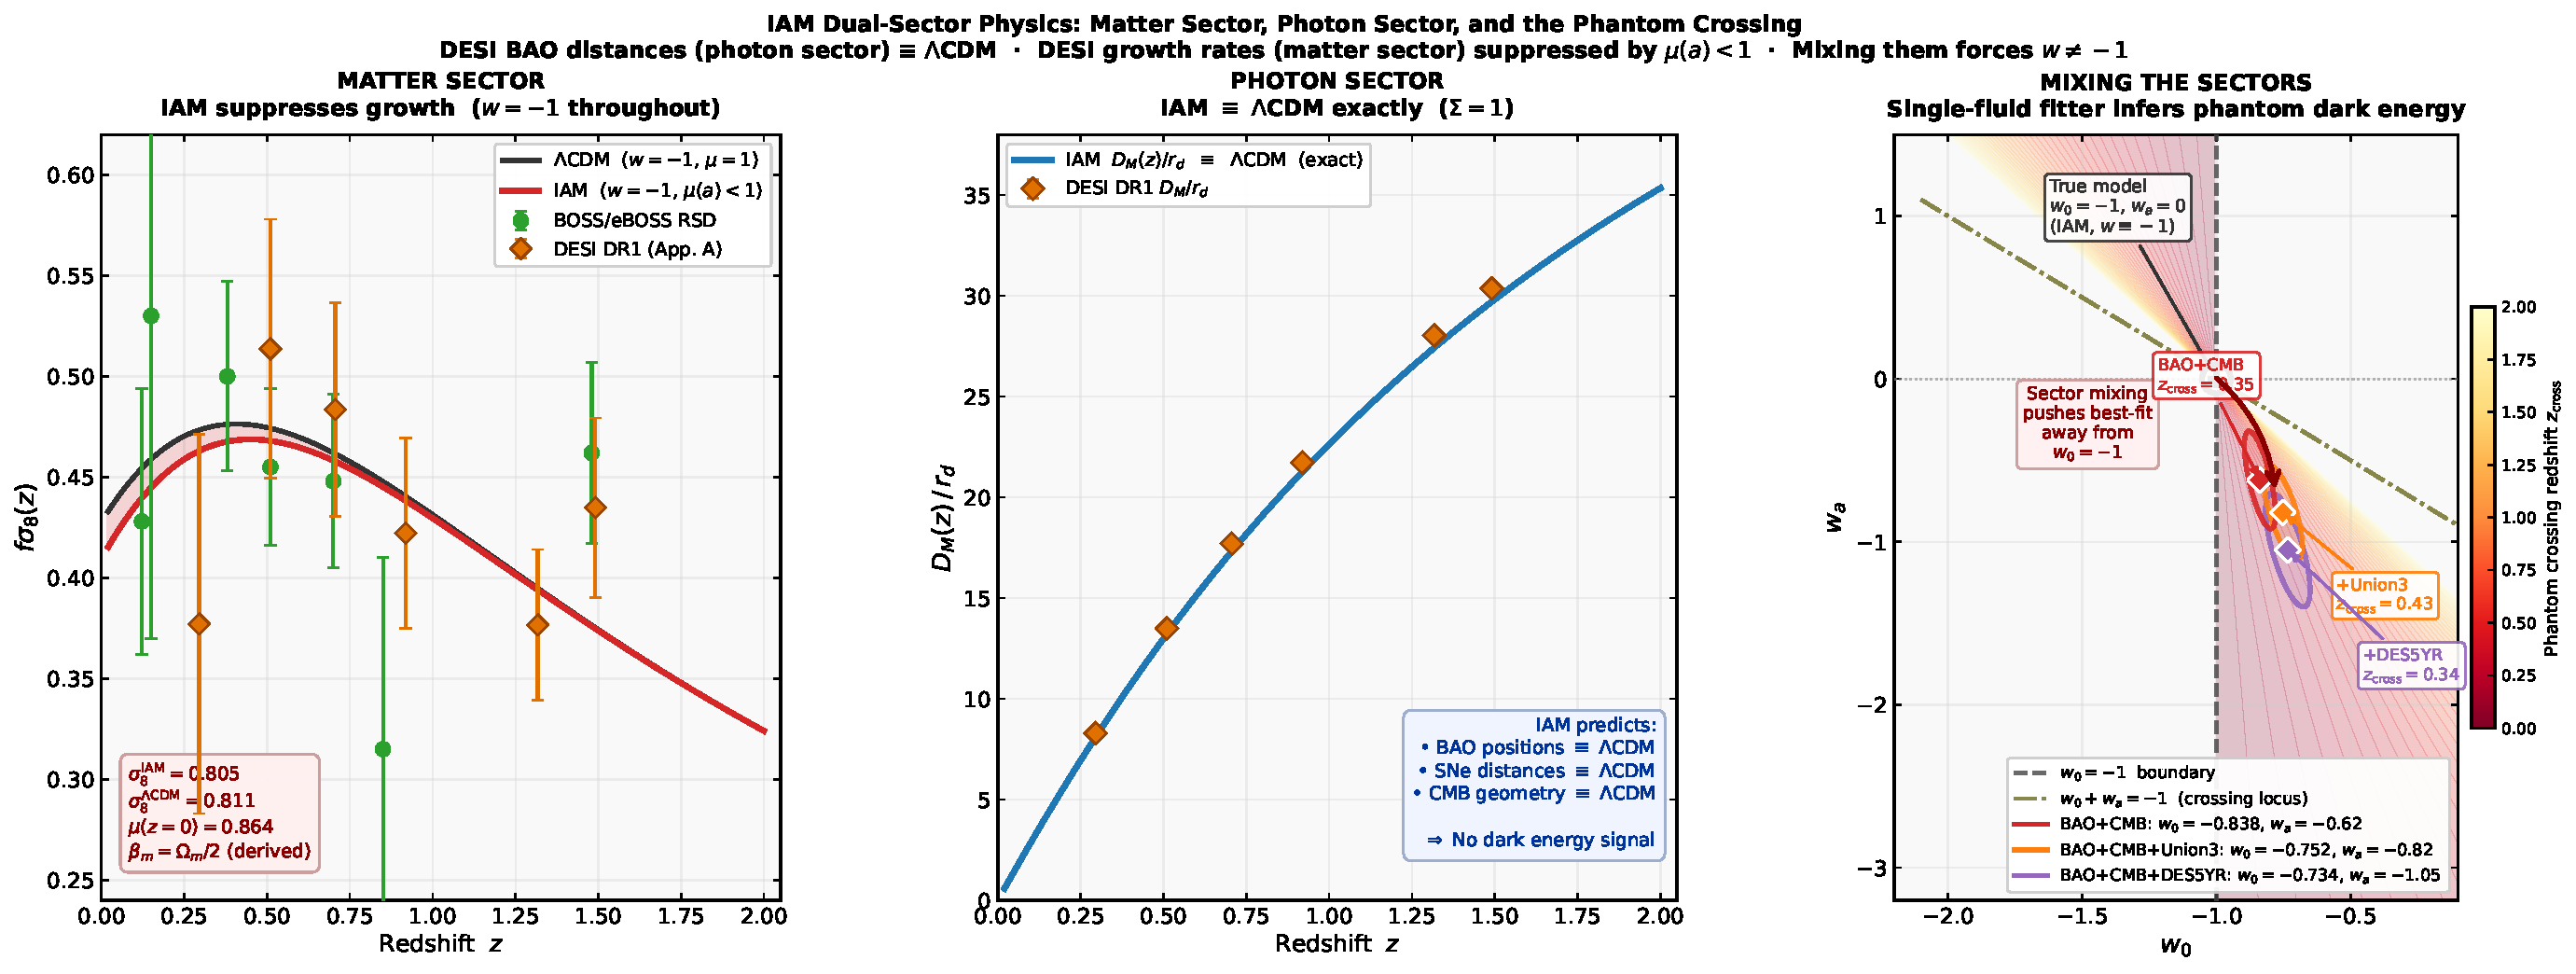
\includegraphics[width=\textwidth]{iam_sector_phantom.pdf}
\caption{
\textbf{Matter sector, photon sector, and the phantom crossing.}
\textit{Left panel (matter sector):} $f\sigma_8(z)$ comparison.
IAM (red, $w = -1$, $\mu(a) < 1$) lies below \lcdm{} (grey) by
$\lesssim 2\%$ at $z \lesssim 0.5$.
Green circles: BOSS/eBOSS RSD compilation~\citep{Beutler2012,Howlett2015,Alam2017boss,Alam2021eboss}.
Orange diamonds: DESI DR1 ShapeFit-only values~\citep{DESI2024DR1FS} (Appendix~A).
\textit{Centre panel (photon sector):} $D_M(z)/r_d$ comparison.
IAM (blue) is identical to \lcdm{} at all redshifts ($\Sigma = 1$ exact).
Orange diamonds: DESI DR1 $D_M/r_d$ measurements (Table~11
of~\citealt{DESI2024DR1FS}).
\textit{Right panel (sector mixing):} The $w_0$-$w_a$ plane.
The true IAM/\lcdm{} model (circle, $w_0 = -1$, $w_a = 0$) is marked.
The three DESI DR2 $1\sigma$ contours~\citep{DESI2025DR2BAO}
(red: BAO+CMB; orange: BAO+CMB+Union3; purple: BAO+CMB+DES5YR)
are displaced from the true model into the phantom region.
Phantom crossing redshifts from Eq.~(\ref{eq:zcross}) are annotated.
The background colormap shows $z_{\rm cross}$ at each $(w_0, w_a)$ point.
The dot-dashed line marks the crossing locus $w_0 + w_a = -1$.
}
\label{fig:sector_phantom}
\end{figure}

\subsection{Distinctive signatures}
\label{sec:signatures}

The sector-assignment interpretation predicts three features that
distinguish it from genuine dynamical dark energy:

\paragraph{Scale independence.}
IAM growth suppression is scale-independent at linear order: the additional
Hubble friction term $\beta_m E(a)$ is a function of time only, with no
scale dependence.
Dynamical dark energy models and most modified gravity theories produce
scale-dependent growth through the dark energy sound horizon or modified
dispersion relation.
The DESI full-shape analysis includes scale-dependent information; a test
of whether the $w_0 w_a$CDM preference persists when only the
time-dependent growth amplitude is varied would constrain this.

\paragraph{$\Sigma = 1$ exactly.}
Lensing-based observables (weak lensing convergence, CMB $C_\ell^{\phi\phi}$,
galaxy-galaxy lensing) are photon-sector observables in IAM.
IAM therefore predicts that the lensing power spectrum, the CMB lensing
amplitude, and the $E_G$ statistic~\citep{Zhang2007EG} are identical to
\lcdm{}.
Dynamical dark energy models that also suppress growth generally modify
$\Sigma$ (through the dark energy perturbation potential), producing
correlated changes in lensing and growth that are in principle distinguishable
from the IAM prediction.
Specifically, the ratio $f\sigma_8 / (\Sigma \sigma_8)$ measured by
Euclid cross-correlations will equal $f_{\rm IAM}$ if IAM is correct,
and will differ if $\Sigma \neq 1$.

\paragraph{The Hubble split.}
IAM derives a matter-sector Hubble constant $H_0^{\rm matter} = H_0
\sqrt{1 + \beta_m} = 72.26$~\kms{}, consistent with SH0ES
($73.04 \pm 1.04$~\kms) at $0.75\sigma$.
The photon-sector $H_0 = 67.16 \pm 0.47$~\kms{} is consistent with
Planck ($67.36 \pm 0.54$) at $0.37\sigma$.
A genuine $w \neq -1$ dark energy does not predict the Hubble tension
magnitude; the IAM phantom crossing, the $S_8$ shift, and the
Hubble tension all follow from the single derived parameter $\beta_m$.


%% ─── 6. DISCUSSION ───────────────────────────────────────────────────────────
\section{Discussion}
\label{sec:discussion}

\subsection{Relation to \citet{Ocolgain2024} and \citet{Ocolgain2025}}
\label{sec:ocolgain}

\citet{Ocolgain2024} examined the internal consistency of DESI DR1
$w_0 w_a$CDM fits across different dataset subsets, arguing that the
dark energy preference may be driven by internal tensions in the combined
dataset rather than a genuine cosmological signal.
\citet{Ocolgain2025} found that the DR2 constraints shift significantly
relative to DR1 in a manner that is difficult to reconcile with stable
dynamical dark energy.

The IAM sector-assignment hypothesis is consistent with these observations
and provides a specific physical mechanism.
In IAM, the apparent tension between distance data and growth data is not
a statistical fluctuation but a predicted consequence of the perturbation-only
friction term.
The tension is expected to grow as data improve (because error bars on
$f\sigma_8$ and $D_M/r_d$ shrink at different rates), and the phantom
crossing parameters are expected to shift between dataset combinations
(because each combination weights the photon and matter sectors differently).
Both features are present in the DESI DR1-to-DR2 evolution described
by~\citet{Ocolgain2025}.

\subsection{Comparison with modified gravity models}
\label{sec:mg}

The IAM combination $\mu < 1$, $\Sigma = 1$ is unusual within the
landscape of modified gravity theories~\citep{Pogosian2016}.

$f(R)$ gravity~\citep{Hu2007fR} produces $\mu > 1$ and $\Sigma > 1$.
Horndeski scalar-tensor theories~\citep{Bellini2014} can produce $\mu < 1$
in the Beyond Horndeski regime but generically also modify $\Sigma$.
DGP gravity~\citep{Dvali2000} produces $\mu > 1$.
Interacting dark energy (IDE) models can suppress growth but do so through
a modified dark energy sound horizon that also affects background distances.

The Level~1 Planck MCMC chains, run with the MGCAMB $\mu$-$\Sigma$
parametrisation with both $\mu_0$ and $\Sigma_0$ floating, constrain
$\mu_0 = 0.033 \pm 0.125$ (Planck + RSD).
IAM predicts $\mu_0 = -0.136$, lying $1.3\sigma$ from the posterior peak.
Current CMB and RSD data are insufficient to discriminate between GR and
the IAM prediction at the predicted level.
The Euclid survey, projected to achieve $\sigma(\mu_0) \approx 0.04$ with
$\Sigma$ marginalised~\citep{Euclid2020forecast}, will provide the
decisive test: $3.4\sigma$ if $\mu_0 = -0.136$ is confirmed.

It is important to note that the $\mu < 1$, $\Sigma = 1$ combination is
not achievable in any currently published Horndeski or f(R) framework
without introducing ad hoc conditions.
It arises in IAM as a direct consequence of the null-vs-timelike
decoherence argument, not as a parameter choice.

\subsection{Limitations}
\label{sec:limits}

Several limitations of the analysis presented here should be noted.

\textit{Simplified growth calculation.}
The growth ODE (Section~\ref{sec:growth_calc}) is a simplified treatment
that does not capture the full Boltzmann hierarchy.
The rigorous IAM prediction comes from the Level~2 MCMC (17 converged
chains), which gives $\sigma_8 = 0.7998 \pm 0.0058$.
The standalone ODE overestimates $\sigma_8$ by $0.6\%$ relative to the
Boltzmann result.
All $f\sigma_8$ predictions in Table~\ref{tab:fsig8_full} carry this
caveat; they are accurate to the level required for current data precision
but would need the full Boltzmann calculation for precision comparisons
at $\lesssim 1\%$.

\textit{Qualitative phantom crossing argument.}
The sector-mixing mechanism in Section~\ref{sec:phantom} establishes
the direction and approximate scale of the expected $w_0 w_a$CDM
displacement but does not constitute a likelihood analysis of the full
DESI pipeline.
A rigorous demonstration would require running the DESI full-shape
likelihood with sector-dependent models, treating photon-sector and
matter-sector observables with the appropriate effective expansion rates.
This is computationally feasible using the existing Level~2 CAMB
implementation but requires a dedicated analysis of the DESI datavectors.

\textit{$S_8$ comparison at fixed $\Omega_m$.}
The weak lensing comparison in Section~\ref{sec:lensing} uses survey
$S_8$ values reported at Planck~2018 $\Omega_m$.
Under the IAM dual-sector mechanism, the matter-sector $\Omega_m$ that
weak lensing surveys measure is smaller than the CMB-derived value.
A rigorous $S_8$ comparison would require reprocessing the survey
likelihoods under the modified cosmology.
This is conserved for future work; the comparison in Table~\ref{tab:s8}
uses the apples-to-apples IAM prediction at Planck $\Omega_m$.

\textit{No covariance between $f\sigma_8$ bins.}
The DESI DR1 $f\sigma_8$ values in Table~\ref{tab:fsig8_full} are treated
as independent measurements.
The published DESI DR1 covariance matrix~\citep{DESI2024DR1FS} should be
used for any $\chi^2$ analysis; the pull statistics reported here are
indicative only.


%% ─── 7. CONCLUSIONS ──────────────────────────────────────────────────────────
\section{Conclusions}
\label{sec:conclusions}

We have confronted the Informational Actualization Model against DESI DR1
full-shape $f\sigma_8(z)$ measurements at six redshift bins, DESI DR1 BAO
distances, joint weak lensing $S_8$ constraints from KiDS-Legacy, DES~Y3,
and HSC~Y3, and the DESI DR2 phantom crossing parameters.
The central argument is that the DESI preference for dynamical dark energy is
consistent with --- and specifically predicted by --- the IAM sector-assignment
mechanism, in which matter and photon observables probe physically distinct
effective expansion rates.

The principal findings are:

\begin{enumerate}
\item IAM $f\sigma_8(z)$ predictions are consistent with DESI DR1 ShapeFit
  measurements at all six bins ($0.295 \leq z_{\rm eff} \leq 1.491$),
  with residuals ranging from $-0.87\sigma$ to $+1.42\sigma$.
  The suppression is $\lesssim 2\%$ relative to \lcdm{} at low $z$
  and diminishes to $< 1\%$ above $z \approx 1.3$.

\item IAM $D_M(z)/r_d$ predictions are identical to \lcdm{} at all DESI
  redshifts, consistent with $\Sigma(a) = 1$ derived from the null-worldline
  argument.
  The DESI DR1 $D_M/r_d$ data are consistent with the prediction at all bins.

\item The IAM $\sigma_8 = 0.7998 \pm 0.0058$ (Level~2 MCMC) is consistent
  with the 2025 joint lensing analysis $\sigma_8 = 0.802 \pm 0.020$ at
  $0.1\sigma$.
  Individual KiDS-Legacy, DES~Y3, and HSC~Y3 $S_8$ values remain
  $\approx 2$--$2.5\sigma$ below the IAM prediction when compared at
  Planck~2018 $\Omega_m$.

\item The DESI DR2 phantom crossing ($z_{\rm cross} = 0.33$--$0.43$,
  depending on supernova compilation) falls in the redshift range where
  the IAM growth suppression is $7$--$8\%$, consistent with the
  sector-mixing mechanism.
  Under IAM, $w \equiv -1$ throughout; the apparent phantom crossing is
  an artifact of applying a single-fluid parametrisation to observables
  from two physically distinct sectors.

\item Under the full Planck~2018 likelihood, IAM and \lcdm{} are
  statistically indistinguishable ($\Dchi = +0.54$ best-fit, 17 converged
  MCMC chains, $R-1 < 0.01$).
  The coupling constant $\beta_m = 0.1577$ is recovered by the Planck
  posterior at $0.2\sigma$ without fitting.
\end{enumerate}

The sector-assignment interpretation of the DESI phantom crossing makes
two near-term falsifiable predictions:

\begin{itemize}
\item \textbf{Euclid $\mu$-$\Sigma$ measurement.}
  IAM predicts $\mu_0 = -0.136$ with $\Sigma_0 = 0$ exactly.
  Euclid is projected to measure $\mu_0$ to $\sigma(\mu_0) \approx 0.04$
  with $\Sigma$ marginalised~\citep{Euclid2020forecast}, placing the IAM
  prediction at $3.4\sigma$ significance.
  The simultaneous constraint $\Sigma_0 = 0$ (measured via CMB lensing
  and weak lensing convergence ratios) is required to confirm the
  null-sector interpretation.
  If Euclid measures $\mu_0$ consistent with zero at that precision, IAM
  is falsified.

\item \textbf{DESI Year~5 $f\sigma_8(z)$ shape test.}
  IAM predicts a specific curved $f\sigma_8(z)$ ramp set by
  $E(a) = \exp(1-1/a)$, distinguishable from both a constant rescaling
  and the growth history of any $w \neq -1$ model.
  DESI Year~5 full-shape data will provide $\lesssim 1\%$ precision on
  $f\sigma_8(z)$ across $0.1 < z < 1.6$ with independent bins of width
  $\Delta z \approx 0.1$.
  At that precision, the curved IAM ramp ($7.9\%$ suppression at $z = 0.3$,
  decreasing to $0.6\%$ at $z = 1.5$) is distinguishable from both
  \lcdm{} and the growth history expected for the DESI DR2 best-fit
  $w_0 w_a$CDM parameters.
\end{itemize}

%% ─── ACKNOWLEDGEMENTS ────────────────────────────────────────────────────────
\section*{Acknowledgements}

The author thanks the Planck, SDSS/BOSS/eBOSS, SH0ES, and DESI collaborations
for making their data publicly available.
The CAMB team~\citep{Lewis2011camb} for the Boltzmann solver (v1.5.8).
The MGCAMB team~\citep{mgcamb} for the modified gravity extension.
The Cobaya team~\citep{cobaya} for the MCMC sampling framework.
Analysis scripts, all converged MCMC chains, and the modified Fortran
source (\texttt{equations\_iam\_level2.f90}) are archived at
\url{https://github.com/hmahaffeyges/IAM-Validation}
(Zenodo DOI: \href{https://doi.org/10.5281/zenodo.18702042}{10.5281/zenodo.18702042}).




%% ─── BIBLIOGRAPHY ────────────────────────────────────────────────────────────
\clearpage

\begin{thebibliography}{99}

\bibitem[Aghanim et al.(2020)]{Planck2018params}
Aghanim N., et al. ({Planck Collaboration}), 2020, A\&A, 641, A6.
\newblock \doi{10.1051/0004-6361/201833910}

\bibitem[Aghanim et al.(2020b)]{Planck2018lens}
Aghanim N., et al. ({Planck Collaboration}), 2020b, A\&A, 641, A8.
\newblock \doi{10.1051/0004-6361/201833886}

\bibitem[Alam et al.(2017)]{Alam2017boss}
Alam S., et al., 2017, MNRAS, 470, 2617.
\newblock \doi{10.1093/mnras/stx721}

\bibitem[Alam et al.(2021)]{Alam2021eboss}
Alam S., et al., 2021, Phys.\ Rev.\ D, 103, 083533.
\newblock \doi{10.1103/PhysRevD.103.083533}

\bibitem[Asgari et al.(2021)]{Asgari2021kids}
Asgari M., et al., 2021, A\&A, 645, A104.
\newblock \doi{10.1051/0004-6361/202039070}

\bibitem[Bellini \& Sawicki(2014)]{Bellini2014}
Bellini E., Sawicki I., 2014, JCAP, 07, 050.
\newblock \doi{10.1088/1475-7516/2014/07/050}

\bibitem[B\'{e}rut et al.(2012)]{Berut2012}
B\'{e}rut A., Arakelyan A., Petrosyan A., Ciliberto S., Dillenschneider R.,
Lutz E., 2012, Nature, 483, 187.
\newblock \doi{10.1038/nature10872}

\bibitem[Beutler et al.(2012)]{Beutler2012}
Beutler F., et al., 2012, MNRAS, 423, 3430.
\newblock \doi{10.1111/j.1365-2966.2012.21136.x}

\bibitem[Bousso(2002)]{Bousso2002}
Bousso R., 2002, Rev.\ Mod.\ Phys., 74, 825.
\newblock \doi{10.1103/RevModPhys.74.825}

\bibitem[Cai \& Kim(2005)]{CaiKim2005}
Cai R.-G., Kim S.~P., 2005, JHEP, 02, 050.
\newblock \doi{10.1088/1126-6708/2005/02/050}

\bibitem[de Mattia et al.(2021)]{deMattia2021}
de Mattia A., et al., 2021, MNRAS, 501, 5616.
\newblock \doi{10.1093/mnras/staa3891}

\bibitem[{DESI Collaboration} et al.(2025a)]{DESI2024DR1BAO}
{DESI Collaboration}, Adame A.~G., et al., 2025a, JCAP, 2025, 021.
\newblock \doi{10.1088/1475-7516/2025/07/021}

\bibitem[{DESI Collaboration} et al.(2025b)]{DESI2024DR1cosmo}
{DESI Collaboration}, Adame A.~G., et al., 2025b, JCAP, 2025, 028.
\newblock \doi{10.1088/1475-7516/2025/07/028}

\bibitem[{DESI Collaboration} et al.(2025c)]{DESI2024DR1FS}
{DESI Collaboration}, Adame A.~G., et al., 2025c, JCAP, 2025, 008.
\newblock \doi{10.1088/1475-7516/2025/09/008}

\bibitem[{DESI Collaboration} et al.(2025d)]{DESI2025DR2BAO}
{DESI Collaboration}, Abdul-Karim M., et al., 2025d, Phys.\ Rev.\ D, 112, 083515.
\newblock \doi{10.1103/tr6y-kpc6}

\bibitem[Abbott et al.(2022)]{Abbott2022desy3}
Abbott T.~M.~C., et al. ({DES Collaboration}), 2022, Phys.\ Rev.\ D, 105, 023520.
\newblock \doi{10.1103/PhysRevD.105.023520}

\bibitem[{Euclid Collaboration} et al.(2020)]{Euclid2020forecast}
{Euclid Collaboration}, Blanchard A., et al., 2020, A\&A, 642, A191.
\newblock \doi{10.1051/0004-6361/202038071}

\bibitem[Freedman et al.(2024)]{Freedman2025}
Freedman W.~L., et al., 2024, ApJ, 919, 16.
\newblock \doi{10.3847/1538-4357/ac7c74}

\bibitem[Hou et al.(2021)]{Hou2021}
Hou J., et al., 2021, MNRAS, 500, 1201.
\newblock \doi{10.1093/mnras/staa3234}

\bibitem[Howlett et al.(2015)]{Howlett2015}
Howlett C., et al., 2015, MNRAS, 449, 848.
\newblock \doi{10.1093/mnras/stu2693}

\bibitem[Hu \& Sawicki(2007)]{Hu2007fR}
Hu W., Sawicki I., 2007, Phys.\ Rev.\ D, 76, 064004.
\newblock \doi{10.1103/PhysRevD.76.064004}

\bibitem[Jacobson(1995)]{Jacobson1995}
Jacobson T., 1995, Phys.\ Rev.\ Lett., 75, 1260.
\newblock \doi{10.1103/PhysRevLett.75.1260}

\bibitem[Landauer(1961)]{Landauer1961}
Landauer R., 1961, IBM J.\ Res.\ Dev., 5, 183.
\newblock \doi{10.1147/rd.53.0183}

\bibitem[Lewis \& Bridle(2002)]{Lewis2011camb}
Lewis A., Bridle S., 2002, Phys.\ Rev.\ D, 66, 103511.
\newblock \doi{10.1103/PhysRevD.66.103511}

\bibitem[Li et al.(2023)]{Li2023hsc}
Li X., et al., 2023, Phys.\ Rev.\ D, 108, 123518.
\newblock \doi{10.1103/PhysRevD.108.123518}

\bibitem[Mahaffey(2026)]{Mahaffey2026preprint}
Mahaffey H.~W., 2026, Universe, submitted (ID: universe-4189350).
\newblock Code: \url{https://github.com/hmahaffeyges/IAM-Validation}.
\newblock \doi{10.5281/zenodo.18702042}

\bibitem[\'O~Colg\'ain \& Sheikh-Jabbari(2025)]{Ocolgain2024}
\'O~Colg\'ain E., Sheikh-Jabbari M.~M., 2025, MNRAS Lett., 542, L24.
\newblock \doi{10.1093/mnrasl/slaf055}

\bibitem[\'O~Colg\'ain et al.(2025)]{Ocolgain2025}
\'O~Colg\'ain E., et al., 2025, preprint (arXiv:2504.04417).

\bibitem[Pogosian \& Silvestri(2016)]{Pogosian2016}
Pogosian L., Silvestri A., 2016, Phys.\ Rev.\ D, 94, 104014.
\newblock \doi{10.1103/PhysRevD.94.104014}

\bibitem[Riess et al.(2022)]{Riess2022}
Riess A.~G., et al., 2022, ApJL, 934, L7.
\newblock \doi{10.3847/2041-8213/ac5c5b}

\bibitem[Shannon(1948)]{Shannon1948}
Shannon C.~E., 1948, Bell Syst.\ Tech.\ J., 27, 379.
\newblock \doi{10.1002/j.1538-7305.1948.tb01338.x}

\bibitem[Sheth \& Tormen(1999)]{ShethTormen1999}
Sheth R.~K., Tormen G., 1999, MNRAS, 308, 119.
\newblock \doi{10.1046/j.1365-8711.1999.02692.x}

\bibitem[St\"olzner et al.(2025)]{Stolzner2025kids}
St\"olzner B., et al., 2025, A\&A, in press (arXiv:2503.19442).

\bibitem[Torrado \& Lewis(2021)]{cobaya}
Torrado J., Lewis A., 2021, JCAP, 05, 057.
\newblock \doi{10.1088/1475-7516/2021/05/057}

\bibitem[Wang et al.(2023)]{mgcamb}
Wang Z., et al., 2023, JCAP, 2023, 022.
\newblock \doi{10.1088/1475-7516/2023/10/022}

\bibitem[Wong et al.(2020)]{Wong2020}
Wong K.~C., et al., 2020, MNRAS, 498, 1420.
\newblock \doi{10.1093/mnras/stz3094}

\bibitem[Wright et al.(2025)]{Wright2025kids}
Wright A.~H., et al., 2025, A\&A, in press (arXiv:2503.19441).

\bibitem[Zhang et al.(2007)]{Zhang2007EG}
Zhang P., Liguori M., Bean R., Dodelson S., 2007, Phys.\ Rev.\ Lett., 99, 141302.
\newblock \doi{10.1103/PhysRevLett.99.141302}

\bibitem[Dvali, Gabadadze \& Porrati(2000)]{Dvali2000}
Dvali G., Gabadadze G., Porrati M., 2000, Phys.\ Lett.\ B, 485, 208.
\newblock \doi{10.1016/S0370-2693(00)00669-9}

\end{thebibliography}

\end{document}
